\subsection{Label for Each Day}

Since the data are to be reduced into daily records, there is a problem of determining the labels. For the purpose of our project, we have to assign to every observation (i.e. a specific day) a label representing the weather type of the next day based on precipitation data collected from different stations.

According to the U.S. National Weather Service (NWS), the threshold for daily precipitation is usually 0.01 inches (0.25 mm). With such threshold, we may get daily weather type for every station. It is then natural to let them vote for the daily weather type of the city: a day should be viewed as ``a day with precipitation" if and only if the precipitation recorded are more than 0.01 inches for over half of the stations. To make it clear, a specific day should be labeled according to the proportion of the stations recording more than 0.01 inches of precipitation in following day.

Such labels can be justified by showing that it meets the data from NWS pretty well.\footnote{In fact, the voting threshold, i.e. $50\%$, is also determined by minimizing the RSS (residual sum of squares).}

By applying such labels, we may notice that the data set is quite balanced: there are 974 days with precipitation among the 2192 days observed here.

\begin{figure}[h]
\center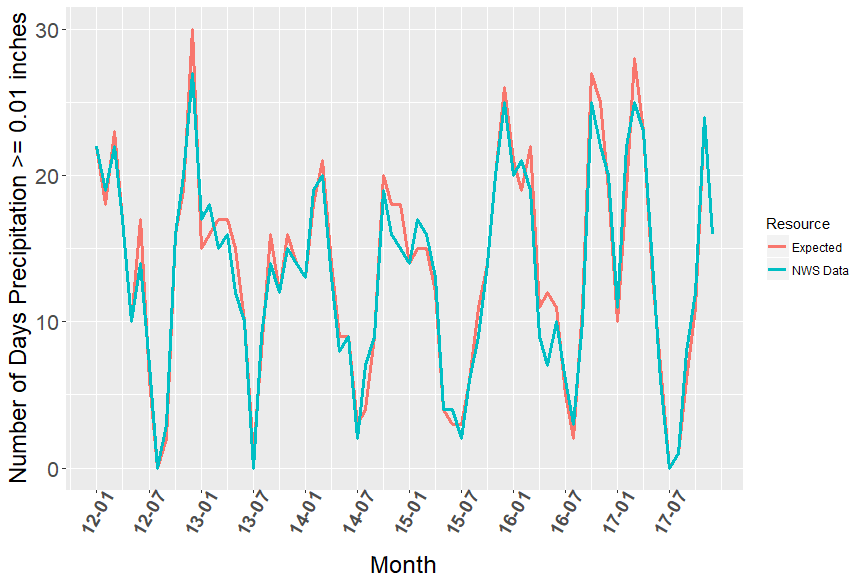
\includegraphics[width = .7\textwidth]{rainyday.png}
\caption{Monthly Number of Days Precipitation \(\geq\) 0.01 Inches}
\label{rainyday}
\end{figure}